\documentclass{templates/homework}

\title{Our Universe Homework 1}
\author{Christoffer Aakre}
\date{29 January 2020}

\begin{document}

\maketitle

\exercise 
\exercisepart
The number of metres in a light year is given by
\begin{align*}
    &\SI{3E8}{\meter\per\second} \times 1 \text{ year} \\
    &= \SI{3E8}{\meter\per\second} \times (3600 \times 24 \times 365) \text{ s} \\
    &= \SI{9.46E15}{\meter}.
\end{align*}
\exercisepart
The light travel time $t$ is given by:
\begin{align*}
    t &= \frac{\text{distance}}{c} \\
    &= \frac{40 \times \SI{1.5E11}{\meter}}{\SI{3E8}{\meter\per\second}} \\
    &= \SI{2E4}{\second} \\
    &\approx \text{5 hours and 33 minutes}.
\end{align*}
\exercisepart
The time $t$ since its launch is given by
\begin{align*}
    t &= \frac{\text{distance}}{\text{speed}} \\
    &= \frac{125 \times \SI{1.5E11}{\meter}}{\SI{17E3}{\meter\per\second}} \\
    &= \SI{1.1E9}{\second} \\
    &= \text{34.97 years} \\
    &\approx \text{35 years}.
\end{align*}
So the launch date should be in $2020 - 35 = 1985$. The actual
lunch date is $1977$.
\begin{subexercises}
    \item \begin{align*}
        t_\text{i} &= \frac{4.3 \times \SI{9.46E15}{\meter}}{\SI{17E3}{\meter\per\second}} \\
        &= \SI{2.39E12}{\second} \\
        &= \SI{7.5876E4}{} \text{ years} \\
        &\approx \text{75880 years}. \\
        \end{align*}
    \item 
    \begin{align*}
        t_\text{ii} &= t_\text{i} \times \frac{10^5}{4.3} \\
        &\approx \SI{1.76E9}{} \text{ years}.
    \end{align*}
    \item
    \begin{align*}
        t_\text{iii} &= t_\text{i} \times \frac{2 \times 10^6}{4.3} \\
        &\approx \SI{3.53E10}{} \text{ years}.
    \end{align*}
\end{subexercises}
\exercisepart
Let the time that passes for the astronaut be $t^\prime$, and the
time that passes for their twin sister be $t$. Then, due to time dilation from special
relativity, we have
\begin{align*}
    t^\prime &= t\sqrt{1 - \frac{v^2}{c^2}} \\
    &= t\sqrt{1 - \frac{0.995^2}{1^2}} \\
    &= t\sqrt{9.975 \times 10^{-3}} \\
    &= t \times 9.987 \times 10^{-2}. \\
\end{align*}
The time $t$ as measured by the twin sister on Earth is
given by
\begin{align*}
    t &= \frac{2 \times 4.3 \text{ lightyears}}{0.995 \times \text{speed of light}} \\
    &= \frac{2 \times 4.3 \text{ years}}{0.995} \\
    &= 8.6432 \text{ years} \\
    &\approx \text{8.6 years}.
\end{align*}
So, the twin sister will be 38 or 39 years old, depending on how far
away her birthday was when the astronaut left Earth. The time $t^\prime$ that passed
for the astronaut is 
\begin{align*}
    &8.6432 \text{ years} \times 9.987 \times 10^{-2} \\
    &= 0.8632 \text{ years} \\
    &\approx \text{about 10 months},
\end{align*}
so the astronaut will be 30 or 31 years old, depending on how far away his birthday was
when he left Earth.
\exercise
\exercisepart
\begin{figure}[t]
    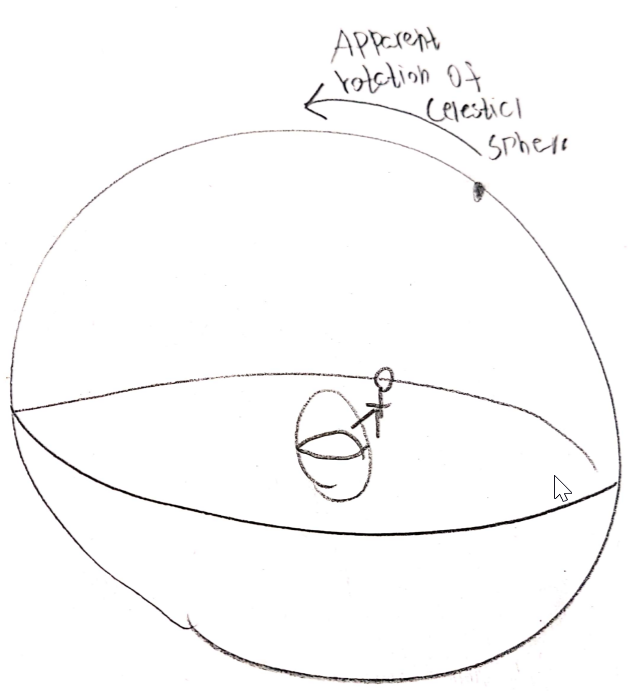
\includegraphics[]{diagrams/figure1.png}
    \caption{The celestial sphere appears to rotate
    around the Earth in the opposite direction of the
    Earth's rotation.}
    \label{fig:1}
\end{figure}
The earth is spinning in the eastward direction. Thus, the
celestial sphere appears to us to spin in the westward direction, and so the stars
in the sky appear to move to the west. Thus, the stars that pass through our zenith
will all have different right ascensions. However, since the earth spins on a plane, there
is no spin in the North or South direction, and so the celestial sphere too does not appear to spin
in the North or South direction. Therefore, the declination value of all the stars that pass
through the zenith will be the same. See \figref{fig:1}
\exercisepart
\begin{figure}[t]
    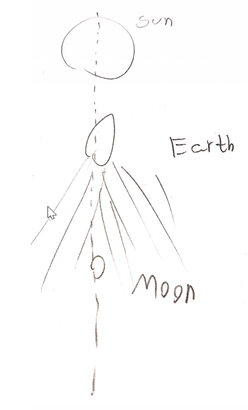
\includegraphics[]{diagrams/rsz_figure2.png}
    \caption{Lunar eclipses occur when the Sun, Earth and Moon line up.
    However, the Moon's orbit is slightly tilted, so they don't always
    line up every month.}
    \label{fig:2}
\end{figure}
A lunar eclipse occurs when the Sun, Earth, and Moon line up,
and the Earth blocks the Sun's light, preventing it from reaching the
Moon, leaving the Moon in the Earth's shadow. So, it would be natural to
expect a lunar eclipse once a month when the Moon lines up behind the Earth.
However, the Moon's orbital plane is tilted slightly relative to the line joining
the centres of the Earth and Sun, and so often, when we would expect a lunar eclipse,
the Moon is actually below or above the Earth, so there is no lunar eclipse.
See \figref{fig:2}
\exercisepart
\begin{figure}[t]
    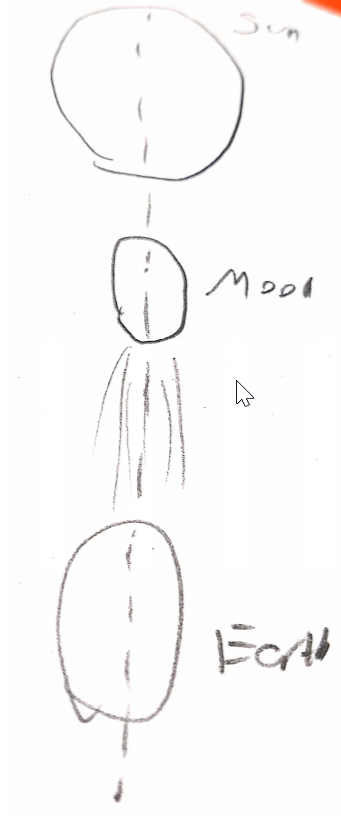
\includegraphics[]{diagrams/figure3.png}
    \caption{A solar eclipse occurs when the Moon blocks
    out the sunlight.}
    \label{fig:3}
\end{figure}
A solar eclipse occurs when the Sun, Moon, and Earth line up, and the Moon
blocks out the sunlight so that the Sun is hidden behind the Moon. The Moon's apparent size
varies with time since the Earth-Moon orbit is elliptical, not circular. Sometimes,
the Moon's apparent size is not large enough to completely cover the Sun, and so a
narrow ring of sun is seen around the Moon's shadow. This is known as an
\textbf{annular eclipse}. See \figref{fig:3}
\exercisepart
\begin{figure}[t]
    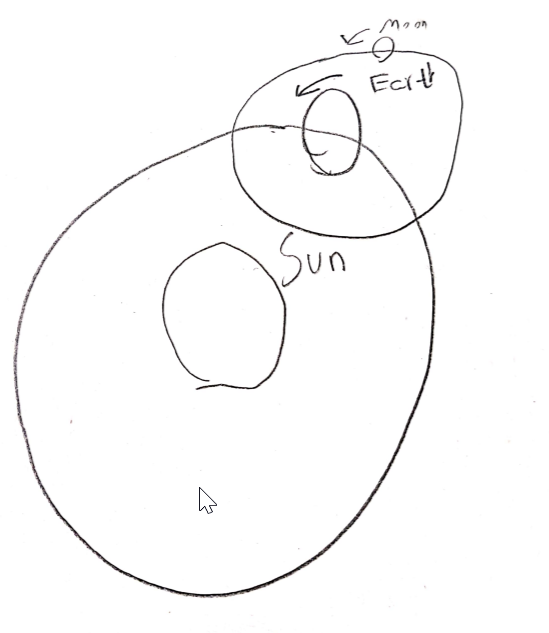
\includegraphics[]{diagrams/figure4.png}
    \caption{By the time the Moon has orbited the Earth,
    the Earth has moved about $30^\circ$ through its orbit around the sun,
    so the Moon needs to \Quote{catch up}.}
    \label{fig:4}
\end{figure}
A \textbf{sidereal month} is the time it takes for the Moon to complete
one orbit around the Earth. It is approximately 27.3 days.

A \textbf{synodic month} is the time between two successive New Moons. It is
approximately 29.5 days. A synodic month is about 8\% longer than a sidereal month
because in the time the month has orbited the Earth one time, the Earth has moved about $30^\circ$ through its
orbit around the sun, and so the Moon must move an extra $30^\circ$ around the Earth before
we get a New Moon. Therefore, in a sidereal month, the Moon moves $360^\circ$, whereas in a synodic month
it moves $390^\circ$, and so the ratio of the synodic month to the sidereal month is given by

\begin{align*}
    \frac{\text{synodic month}}{\text{sidereal month}}
    &= \frac{390^\circ}{360^\circ} \\
    &= \frac{13}{12} \\
    &= 1.08333\dots \\
    &= \text{About 8\% longer}.
\end{align*}
See \figref{fig:4}
\exercise
The Earth is not perfectly spherical, so sometimes
there is a net force on the Earth from the Sun with a component
perpendicular to the plane of the Earth-Sun orbit. 6 months later,
when the Earth is on the opposite side of the Sun, the net force is in the opposite direction,
but the displacement vector from the Earth to the Sun is also in the opposite direction,
and thus the resultant torque is in the same direction in both cases. Thus, the
precession builds up over time. The period of precession is about 26000 years.
One consequence is that the time between consecutive winters
or consecutive summers is about 20 minutes shorter than the time it takes
for the Earth to complete one orbit around the Sun. Also, the pole stars change
with time due to the precession, i.e. Polaris has not always been the North star,
and will not always be.
\end{document}
